% !TEX root = ../00_thesis.tex

%-------------------------------------------------------------------------------
\section{\triscale in Action}
\label{sec:triscale_eval}
%-------------------------------------------------------------------------------

\begin{figure}
    \centering
    \begin{subfigure}{\linewidth}
        \centering
       	\href{\triscalefig{Figure-4}}{
        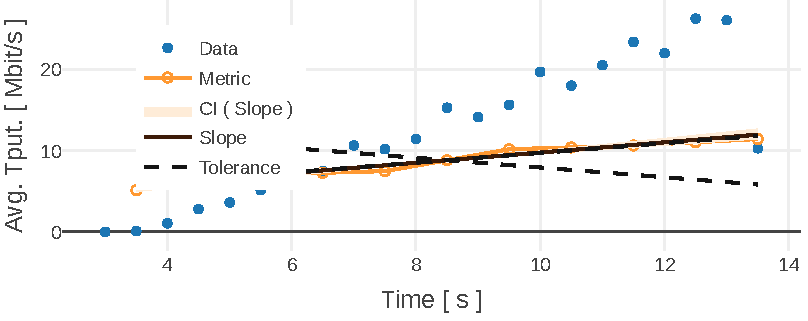
\includegraphics[scale=1]{Figures/plot_ledbat_10_runtime.pdf}}
        \caption{10\s runtime}
        \label{fig:10s}
    \end{subfigure}

    \begin{subfigure}[b]{\linewidth}
        \centering
       	\href{\triscalefig{Figure-4}}{
        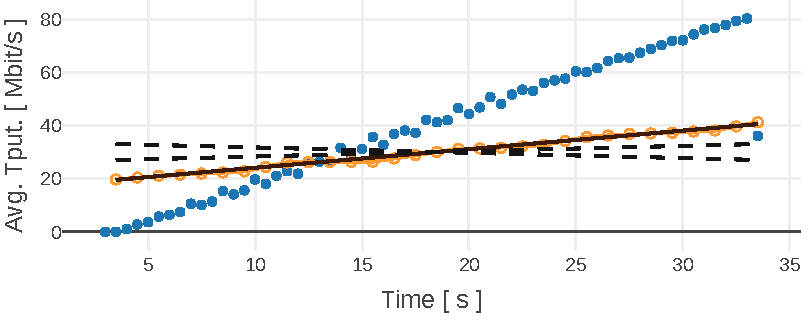
\includegraphics[scale=1]{Figures/plot_ledbat_30_runtime.pdf}}
        \caption{30\s runtime}
        \label{fig:30s}
    \end{subfigure}

    \begin{subfigure}[b]{\linewidth}
        \centering
       	\href{\triscalefig{Figure-4}}{
        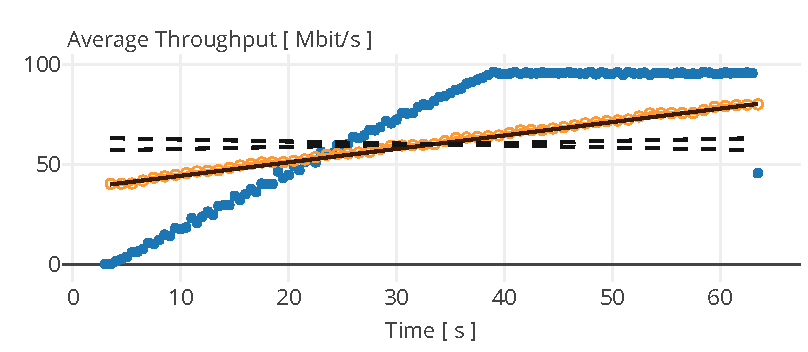
\includegraphics[scale=1]{Figures/plot_ledbat_60_runtime.pdf}}
        \caption{60\s runtime}
        \label{fig:60s}
    \end{subfigure}
    \caption{Egress throughput of \textit{LEDBAT} in MahiMahi, calibrated to the real path from AWS California to Mexico~\cite{yan18pantheon}.
    \capt{\mbox{A runtime} of 30\s is clearly not sufficient for \textit{LEDBAT}'s throughput to converge (\Cref{fig:30s}). The scheme does converge eventually (\Cref{fig:60s}), but even with 60\s runtime, \triscale's convergence test fails: the impact of the start-up phase is too important. Two possible solutions are to (i)~increase the runtime or (ii)~prune the start-up time from the raw data.}}
    \label{fig:ledbat_convergence}
\end{figure}

This section continues the case study introduced in \cref{subsec:triscale_intro_example}.
We compare the performance of 17 congestion-control schemes using Pantheon~\cite{yan18pantheon}. We evaluate the throughput and one-way delay of long-running full-throttle flows, \ie stable flows whose only throttling/limiting factor is the congestion control.
For a fair comparison between the schemes, we use the MahiMahi emulator~\cite{netravali2015mahimahi} (integrated in Pantheon). We focus on a single flow scenario and use the calibrated path from AWS California to Mexico.%
\footnote{\href{https://pantheon.stanford.edu/result/6539/}{pantheon.stanford.edu/result/6539/}}
The complete case study is available as complementary materials~(\cref{append:triscale_artifacts});
we present here only a fraction of it and focus on showcasing how \triscale avoids certain shortcomings in the experiment design and analysis. Finally, we illustrate how to quantify performance variability: a prerequisite for assessing reproducibility (\cref{subsec:reproducibility}).

%-------------------------------------------------------------------------------
\fakepar{Convergence time}
The first step in the design of an evaluation is to decide how long the runs should be.
Since all schemes are different, it is hard to know a priori the minimum runtime for which the various schemes actually converge.

We test runtimes from 10 to 60\s and check whether the 17 congestion-control schemes pass \triscale's convergence test (\cref{subsec:triscale_stats}).
With a runtime of 30\s, only twelve schemes often pass the test; others (\textit{Verus}, \textit{PCC-Allegro}, \textit{Copa}, and \textit{QUIC Cubic}) converge in less than half the runs.
Furthermore, \textit{LEDBAT} never pass the test, even with a runtime of 60\s.
The reason for this is shown in~\Cref{fig:ledbat_convergence}: the inner working of the protocol causes the throughput to ramp-up in the first 38\s of runtime and then converge to about 92\mbps.
If one uses 30\s runtime without checking for convergence, the computed average throughput is about 40\mbps, which is a wrong estimation of \textit{LEDBAT} ``long-running'' throughput.
By performing the convergence test, \triscale hints the experimenter about the need to either increase the runtime, or prune the start-up time in the raw data.

\begin{figure}
    \centering
   	\href{\triscalefig{Figure-5}}{
    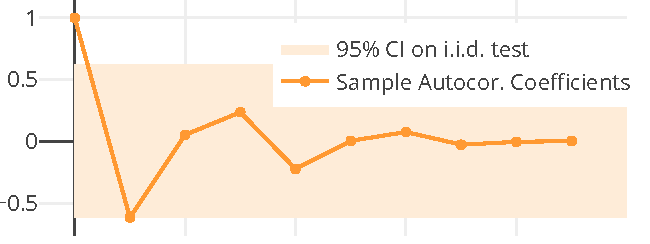
\includegraphics[scale=1]{Figures/plot_webrtc_autocorr_passed.pdf}}\\
   	\href{\triscalefig{Figure-5}}{
    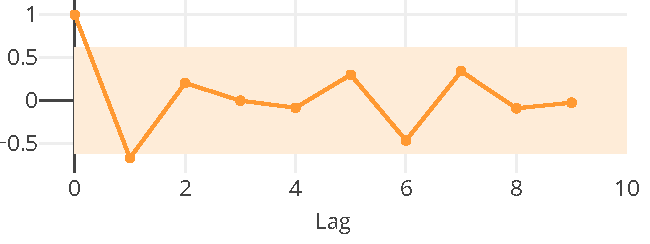
\includegraphics[scale=1]{Figures/plot_webrtc_autocorr_failed.pdf}}
    \caption{Autocorrelation coefficients for two exemplary series of \textit{WebRTC}.
    \capt{The upper series passes the autocorrelation test, whereas the lower series does not: this is an artifact induced by the small number of samples (here: 10 samples).}
    }
    \label{fig:webrtc_autocorr}
\end{figure}

%-------------------------------------------------------------------------------
\fakepar{Independence tests}
The computation of \triscale's KPIs and variability scores requires the samples to be \iid (\cref{subsec:triscale_stats}).
However, the number of runs and series performed in an evaluation tends to be small (as experiments are both time- and resource-consuming), which limits the significance of the independence test.
\Cref{fig:webrtc_autocorr} illustrates this problem: it shows the autocorrelation plot for two series for \textit{WebRTC}.
The autocorrelation coefficients must be in the shaded gray area for the test to pass.
In this case, the upper series passes the test, whereas the lower one does not.
However, there is no clear difference in the correlation structure of the two series: the lower series does not seem significantly more correlated than the upper one.
All other series of \textit{WebRTC} pass the independence test, which hints that the failed series is merely an artifact induced by the small number of runs in the series (in this example, 10 runs per series).
In such cases, it is important that the experimenter critically assesses \triscale's results and increase (when necessary) the number of runs or series to improve the significance of results -- or overrule the test~(discussion in \cref{sec:going_further}).

%-------------------------------------------------------------------------------
\fakepar{Evaluation in emulation}
Using the MahiMahi emulator for the evaluation is expected to be the most favorable setting to test the reproducibility of the congestion-control schemes, since it allows to recreate the exact same test conditions and therefore improves the comparability between the runs.
This however has an unexpected side-effect: while they appear to have a very stable behavior, \emph{TCP BBR} and \emph{TCP Cubic} would always fail the independence test. Actually, these two schemes are designed to use all the available bandwidth and, since MahiMahi artificially sets the latter to a fixed value, the two schemes always reach the exact same throughput.
This leads to the exact same metric values; in other words, the throughput is \emph{perfectly correlated} across runs.
Naturally, this is an artifact of the experiment: the independence test will always fail if all data samples have the same value.

\triscale always computes the KPIs and variability scores, even if the independence test fails. The experimenter is responsible to judge whether there is indeed true correlation in the data, or if one can overrule the test result and proceed with the analysis.
In the example of \emph{TCP BBR} and \emph{TCP Cubic}, one can proceed.

%-------------------------------------------------------------------------------
\fakepar{KPIs}
We illustrated in~\cref{subsec:triscale_intro_example} how \triscale's KPIs allow to unambiguously compare the performance of different schemes.
\Cref{fig:example_triscale} shows the KPI for the average throughput (resp. one-way delay), defined as the estimate of the 25th (resp. 75th) percentile with a 75\% confidence level for 10 runs with 30\s runtime.
We use 30\s to compare with the Pantheon results shown in~\Cref{fig:example_pantheon}).
However, five schemes fail to converge sufficiently often and thus do not appear in~\cref{fig:example_triscale}.

%-------------------------------------------------------------------------------
\fakepar{Variability scores}
Although \triscale's KPIs unambiguously compare the performance of diverse schemes, they only consider one series of runs, which does not indicate how reproducible the results actually are.
\triscale investigates reproducibility using sequels and quantifies the expected variability in the KPI values with a variability score~(\cref{subsec:repeatability}).
In this case study, we define the variability score as the difference between the 75th and 25th percentiles, estimated with 75\% confidence.
We compute the variability scores for our two performance dimensions (average throughput and one-way delay -- \Cref{fig:score_matrix}).
The scores can be interpreted as follows: with 75\% probability, the variability scores (orange bars) give the magnitude of variation expected (shall one perform infinitely many series) in the middle 50\% of KPI values.
Hence the variability score quantifies reproducibility: the larger the score, the less reproducible the results are.

\begin{remark}
  \triscale's variability scores are absolute values with units (\eg in \mbps). Arguably, it may be useful to use relative scores (in percentages) to compare the scores of different protocols.
\end{remark}

%-------------------------------------------------------------------------------
\fakepar{Conclusion}
This case study only considers emulation and one emulated path. As such, it does not aim to fully evaluate the performance of the different congestion-control schemes.
Rather, it illustrates how \triscale may be used for an actual performance evaluation and the importance of carefully choosing the parameters of an experiment; such as the runtime~(\Cref{fig:ledbat_convergence}).
We highlight two important takeaways:
\begin{itemize}
  \item It is important to critically consider \triscale's results: the tests are intentionally conservatives to limit the risk of false positives (\eg not detecting correlation in the data),
  \item It is useful to collect more samples than strictly necessary: it improves the significance of the tests and therefore limits the risk of false negatives.
\end{itemize}

\begin{figure}
    \centering
   	\href{\triscalefig{Figure-6}}{
    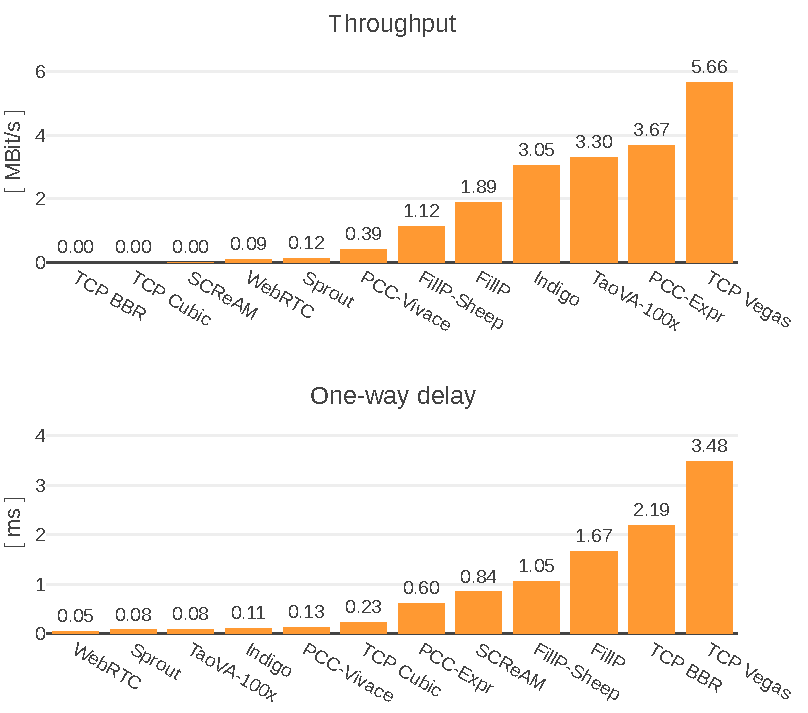
\includegraphics[width=\linewidth]{Figures/plot_score_matrix.pdf}}
    \caption{Variability scores computed by \triscale for the performance dimensions throughput and delay.
    \capt{
      In this example, the variability scores are computed as the 25th to 75th percentile interval estimated with 75\% confidence.
      From the variability scores, the user gets a quantification, with a 75\% probability, of the range of variation in the KPI values for 50\% of the series.
      The variability scores hence quantify reproducibility: the larger the scores, the less reproducible the results are.}
    }
    \label{fig:score_matrix}
\end{figure}
